\documentclass[11pt]{article}
\usepackage{geometry}
\geometry{
 a4paper,
 total={210mm,297mm},
 left=20mm,
 right=20mm,
 top=20mm,
 bottom=20mm,
 }
 
\usepackage[english]{babel}
\usepackage[utf8x]{inputenc}
\usepackage{amsmath}
\usepackage{graphicx}
\usepackage[table,xcdraw]{xcolor}
\usepackage[colorinlistoftodos]{todonotes}
\usepackage{multicol}
\usepackage{ragged2e}
\usepackage{tocloft}
\usepackage{titlesec}
\usepackage{natbib}
\usepackage[parfill]{parskip}
\usepackage{amssymb}
\usepackage{textcomp}
\usepackage{float}
\floatstyle{plain}
\usepackage{color}
\usepackage{epstopdf}
\usepackage{hyperref}
\usepackage{comment}
\hypersetup{
    colorlinks=true,
    linkcolor=blue,
    filecolor=magenta,      
    urlcolor=cyan,
    citecolor=blue
}
\urlstyle{same}
\usepackage{fancyhdr}
\usepackage{lipsum}
\usepackage{subscript}
\usepackage{siunitx}
\usepackage[hypcap]{caption}
\usepackage{capt-of}
\usepackage{wasysym}
\usepackage{wrapfig}
\usepackage{enumitem}
\usepackage{pdflscape}
\usepackage{pdfpages}
\usepackage{csquotes}

%making the bloody title 
\makeatletter
\renewcommand{\maketitle}{\bgroup\setlength{\parindent}{0pt}
\begin{flushleft}
  \textbf{\@title} %the empty line is impt

  \@author
\end{flushleft}\egroup
}
\makeatother

%random things needed
%\renewcommand{\cftsecleader}{\cftdotfill{\cftdotsep}} %let the content table have dots to number
\linespread{1.8}  %making one and a half spacing-sh one and half is actually 1.3
\frenchspacing
%\titlespacing\subsection{0pt}{12pt plus 4pt minus 2pt}{0pt plus 2pt minus 2pt} 
\titlespacing\subsubsection{0pt}{12pt plus 4pt minus 2pt}{0pt plus 2pt minus 2pt} %less spacing between subsubsections
\pagestyle{fancy}
% Set the right side of the footer to be the page number
\fancyhf{} % sets both header and footer to nothing
\renewcommand{\headrulewidth}{0pt}
\fancyfoot[R]{\thepage}
\fancypagestyle{plain}{%
    \renewcommand{\headrulewidth}{0pt}%
    \fancyhf{}%
    \fancyfoot[R]{\thepage}%
}
\setlength{\parskip}{0pt}

%insert title
\title{\textbf{\huge{\textit{pie-1} and its effect on other genes}}}
\date{} 
\author{%
\large{ Jia Le, Lim {  } CID: 00865029 } \\
\textnormal
{\textit{Department of Biology, Imperial College London, South Kensington Campus, London, U.K.}} \\
Submitted: 10 Feb 2017
}

\begin{document}
\maketitle
%space after title
\bigskip

\tableofcontents

\newpage

\section{Introduction}
%what pie-1 is 300 words
%Expression of PIE-1 in HeLa cells has indicated that PIE-1 can inhibit mRNA transcription directly, possibly by targeting a complex that interacts with the CTD of RNAPII
\textit{pie-1} (pharynx and intestine excess) is a maternal effect gene in \textit{Caenorhabditis elegans}. As its name suggests, worms carrying \textit{pie-1} mutations produce embryos with extra pharyngeal and intestinal cells~\citep{Mello1992}. The protein that it encodes, PIE-1, is an embryonic transcriptional repressor that is essential in regulating germ cell fate during the early stages of \textit{C.elegans} development. PIE-1 is a cysteine-X$_{8-10}$-cysteine-X$_{5}$-cysteine-X$_{3}$-histidine (CCCH)-type zinc finger protein that is enriched in germline blastomeres and maintains germ cell fate by inhibiting transcriptional elongation, hence blocking genetic mechanisms responsible for somatic development. PIE-1 may also induce translation of other maternal RNAs such as \textit{nos-2}, which are required for the maintenance of germ cell fate~\citep{Ghosh2008, Gilbert2000, Tenenhaus2001}.
\\
\\
As one of the key transcription factors in germline cells, PIE-1 is likely to interact with many other maternal proteins and mRNA and directly or indirectly repress or activate the transcription of embryonic genes. Nonetheless, most of these interactions has not yet been studied~\citep{Gilbert2000}. Hence, in this practical, likely candidates that interact with PIE-1 up to the first larval stage were identified. Thereafter, such interactions and experimental data that support them, if available, are further clarified in the report.

\section{Methods and Results}

71 possible candidate genes were identified using the list of gene interactions with \textit{pie-1} available on the WormBase. Of which, 7 were promoter regions and were subsequently removed from the list. The expression patterns of the remaining 64 genes were isolated from the dataset obtained from a previous study by \citet{Levin2012}. In \citet{Levin2012}, the relative expression of 19051 genes in \textit{C. elegans} at different time intervals between the 4-cell stage to the first larval stage were estimated using their respective mRNA levels in embryos collected at the corresponding developmental stage~\citep{Levin2012}. 

%Write about the methods you used.  You don't have to give R code, just tell me what packages you used, and if you did anything special tell me what. Nor do you have to use these subsections---they're just examples. 

%400 words
\subsection{\textit{pie-1} expression exponentially decreases during development.}

\begin{figure}[H]
  \centering
    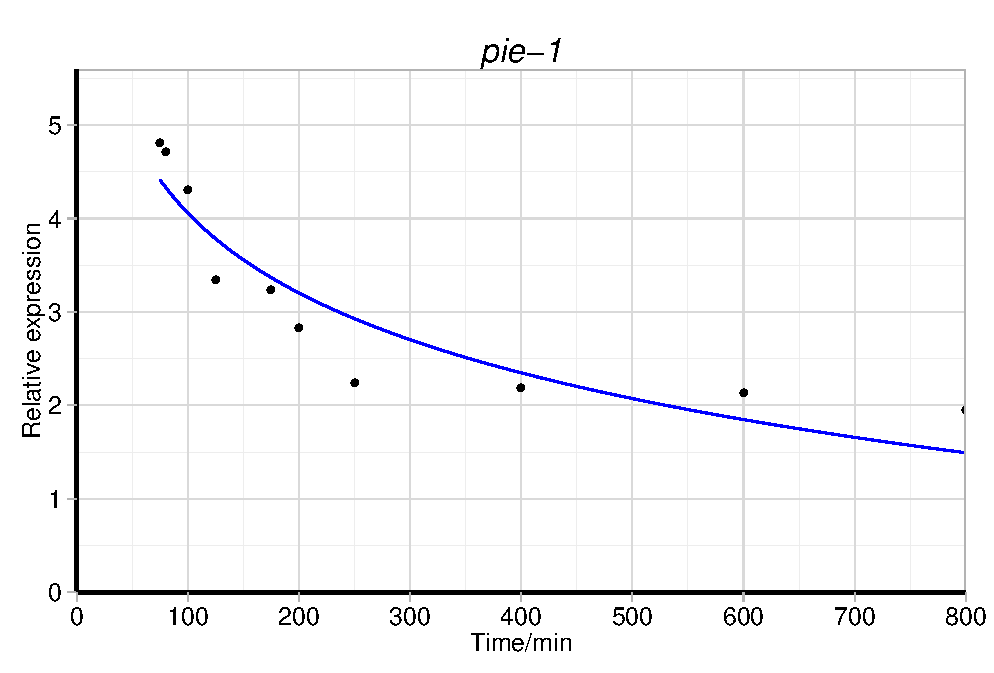
\includegraphics[width=0.8\textwidth]{pie-1_expression.pdf}
  \captionof{figure}{\textbf{Relative expression of \textit{pie-1} during early \textit{C. elegans} development.} \footnotesize Time on the x-axis indicates the amount of time since the 4-cell stage.}
  \label{fig:pie-1_expression}
\end{figure}

As expected, \textit{pie-1} expression level decreases as \textit{C. elegans} embryos proceed to the larval stage~(\autoref{fig:pie-1_expression}). An exponential decay model best fits the relative expression data of \textit{pie-1}~(adj.~r$^2$~=~0.84, intercept~=~9.74$\pm$0.94 , slope~=~-1.23$\pm$0.175, both~p$<$0.001, res. df = 8).

\subsection{Identifying the genes of interest}
\subsubsection{Heatmap and Hierarchal Cluster Analysis}
A heatmap showing the predicted clusters of the 64 candidate genes was generated using Ward's method (ward.D2)~(\autoref{fig:heatmap_general}). 

\begin{figure}[H]
  \centering
    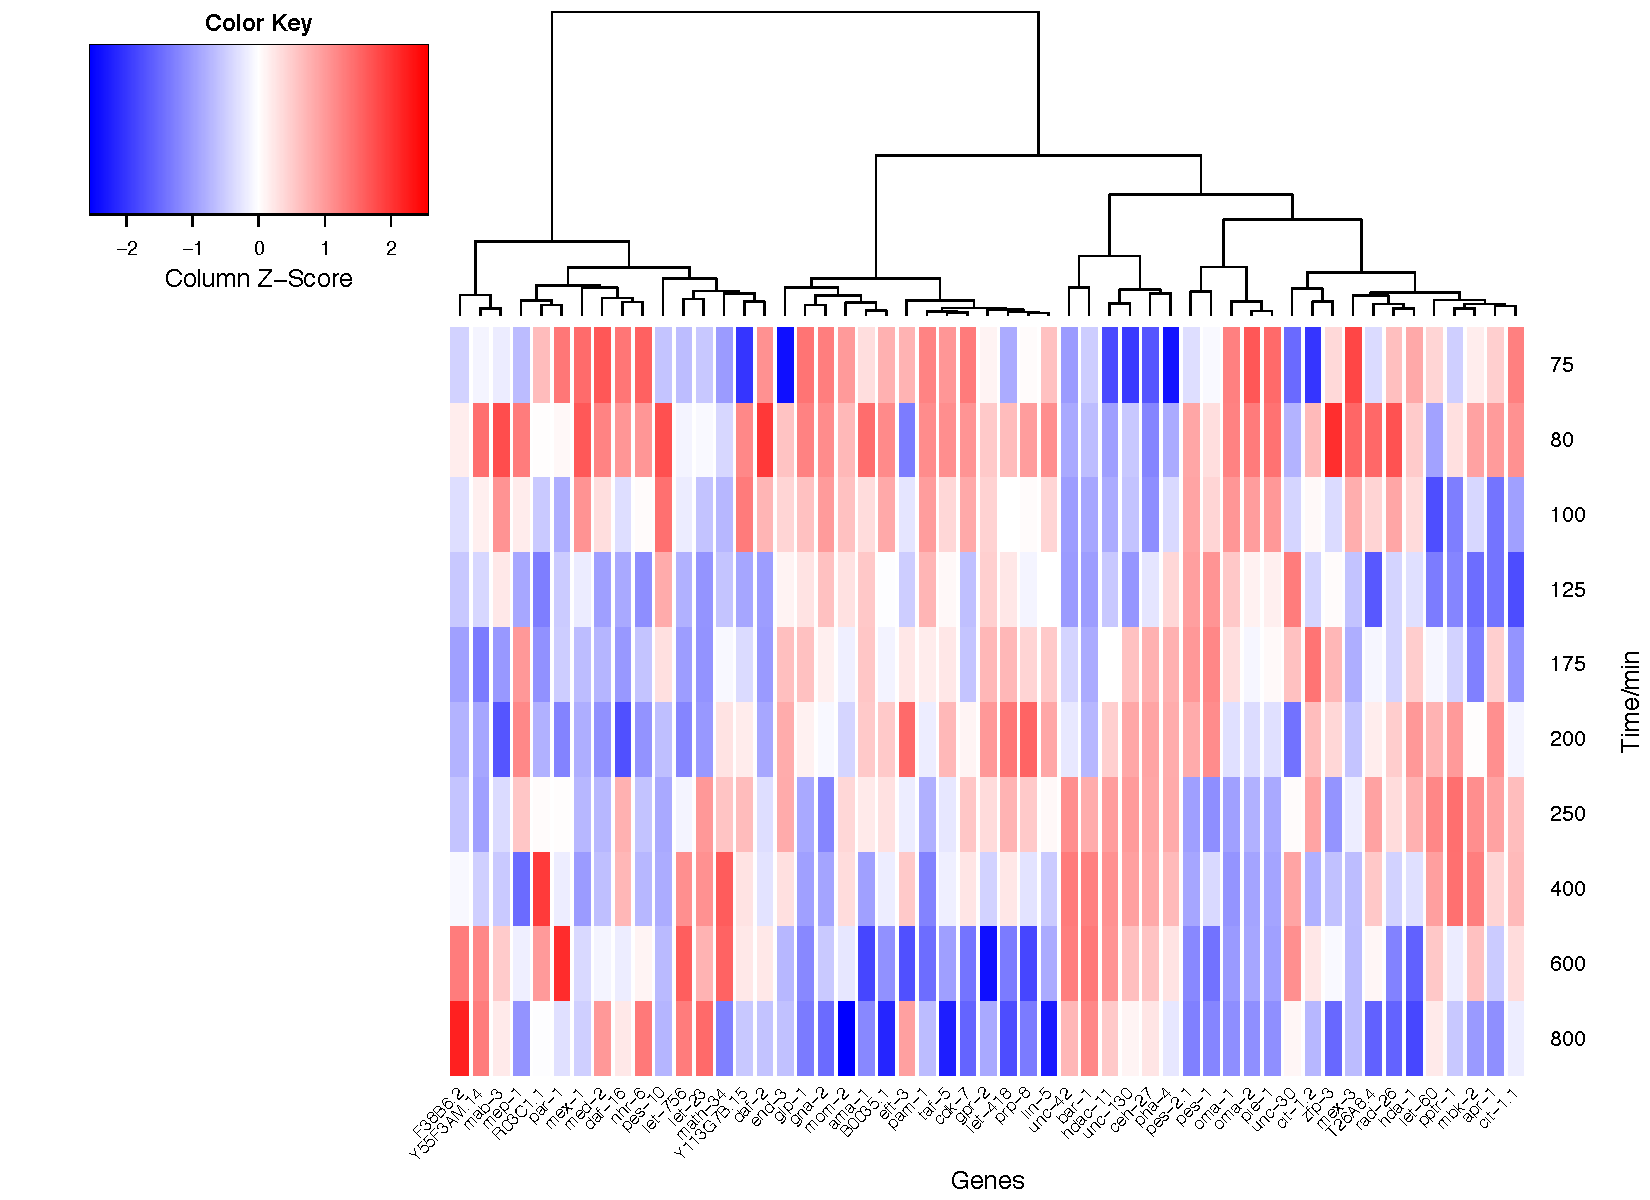
\includegraphics[width=\textwidth]{heatmap_general.pdf}
  \captionof{figure}{\textbf{Heatmap of all 64 candidate genes.}}
  \label{fig:heatmap_general}
\end{figure}

The heatmap~(\autoref{fig:heatmap_general}) does not show consistent expression patterns in clades and was hence not very informative, possibly due to the large number of gene expression patterns used in the analysis.

\subsubsection{Network Construction}
Networks were thus built to isolate a smaller group of genes, which have expression patterns that strongly correlate positively or negatively with that of \textit{pie-1}.
\\
\\
Networks of all 64 genes were constructed using Pearson correlation values of above 0.8. As the community detection algorithm is only able to analyse positive correlation values, two different networks were created. The first network was built using only positive correlations~(\autoref{fig:network_pos}) while the second network was constructed utilising only negative correlations~(\autoref{fig:network_neg}).

\begin{figure}[H]
  \centering
    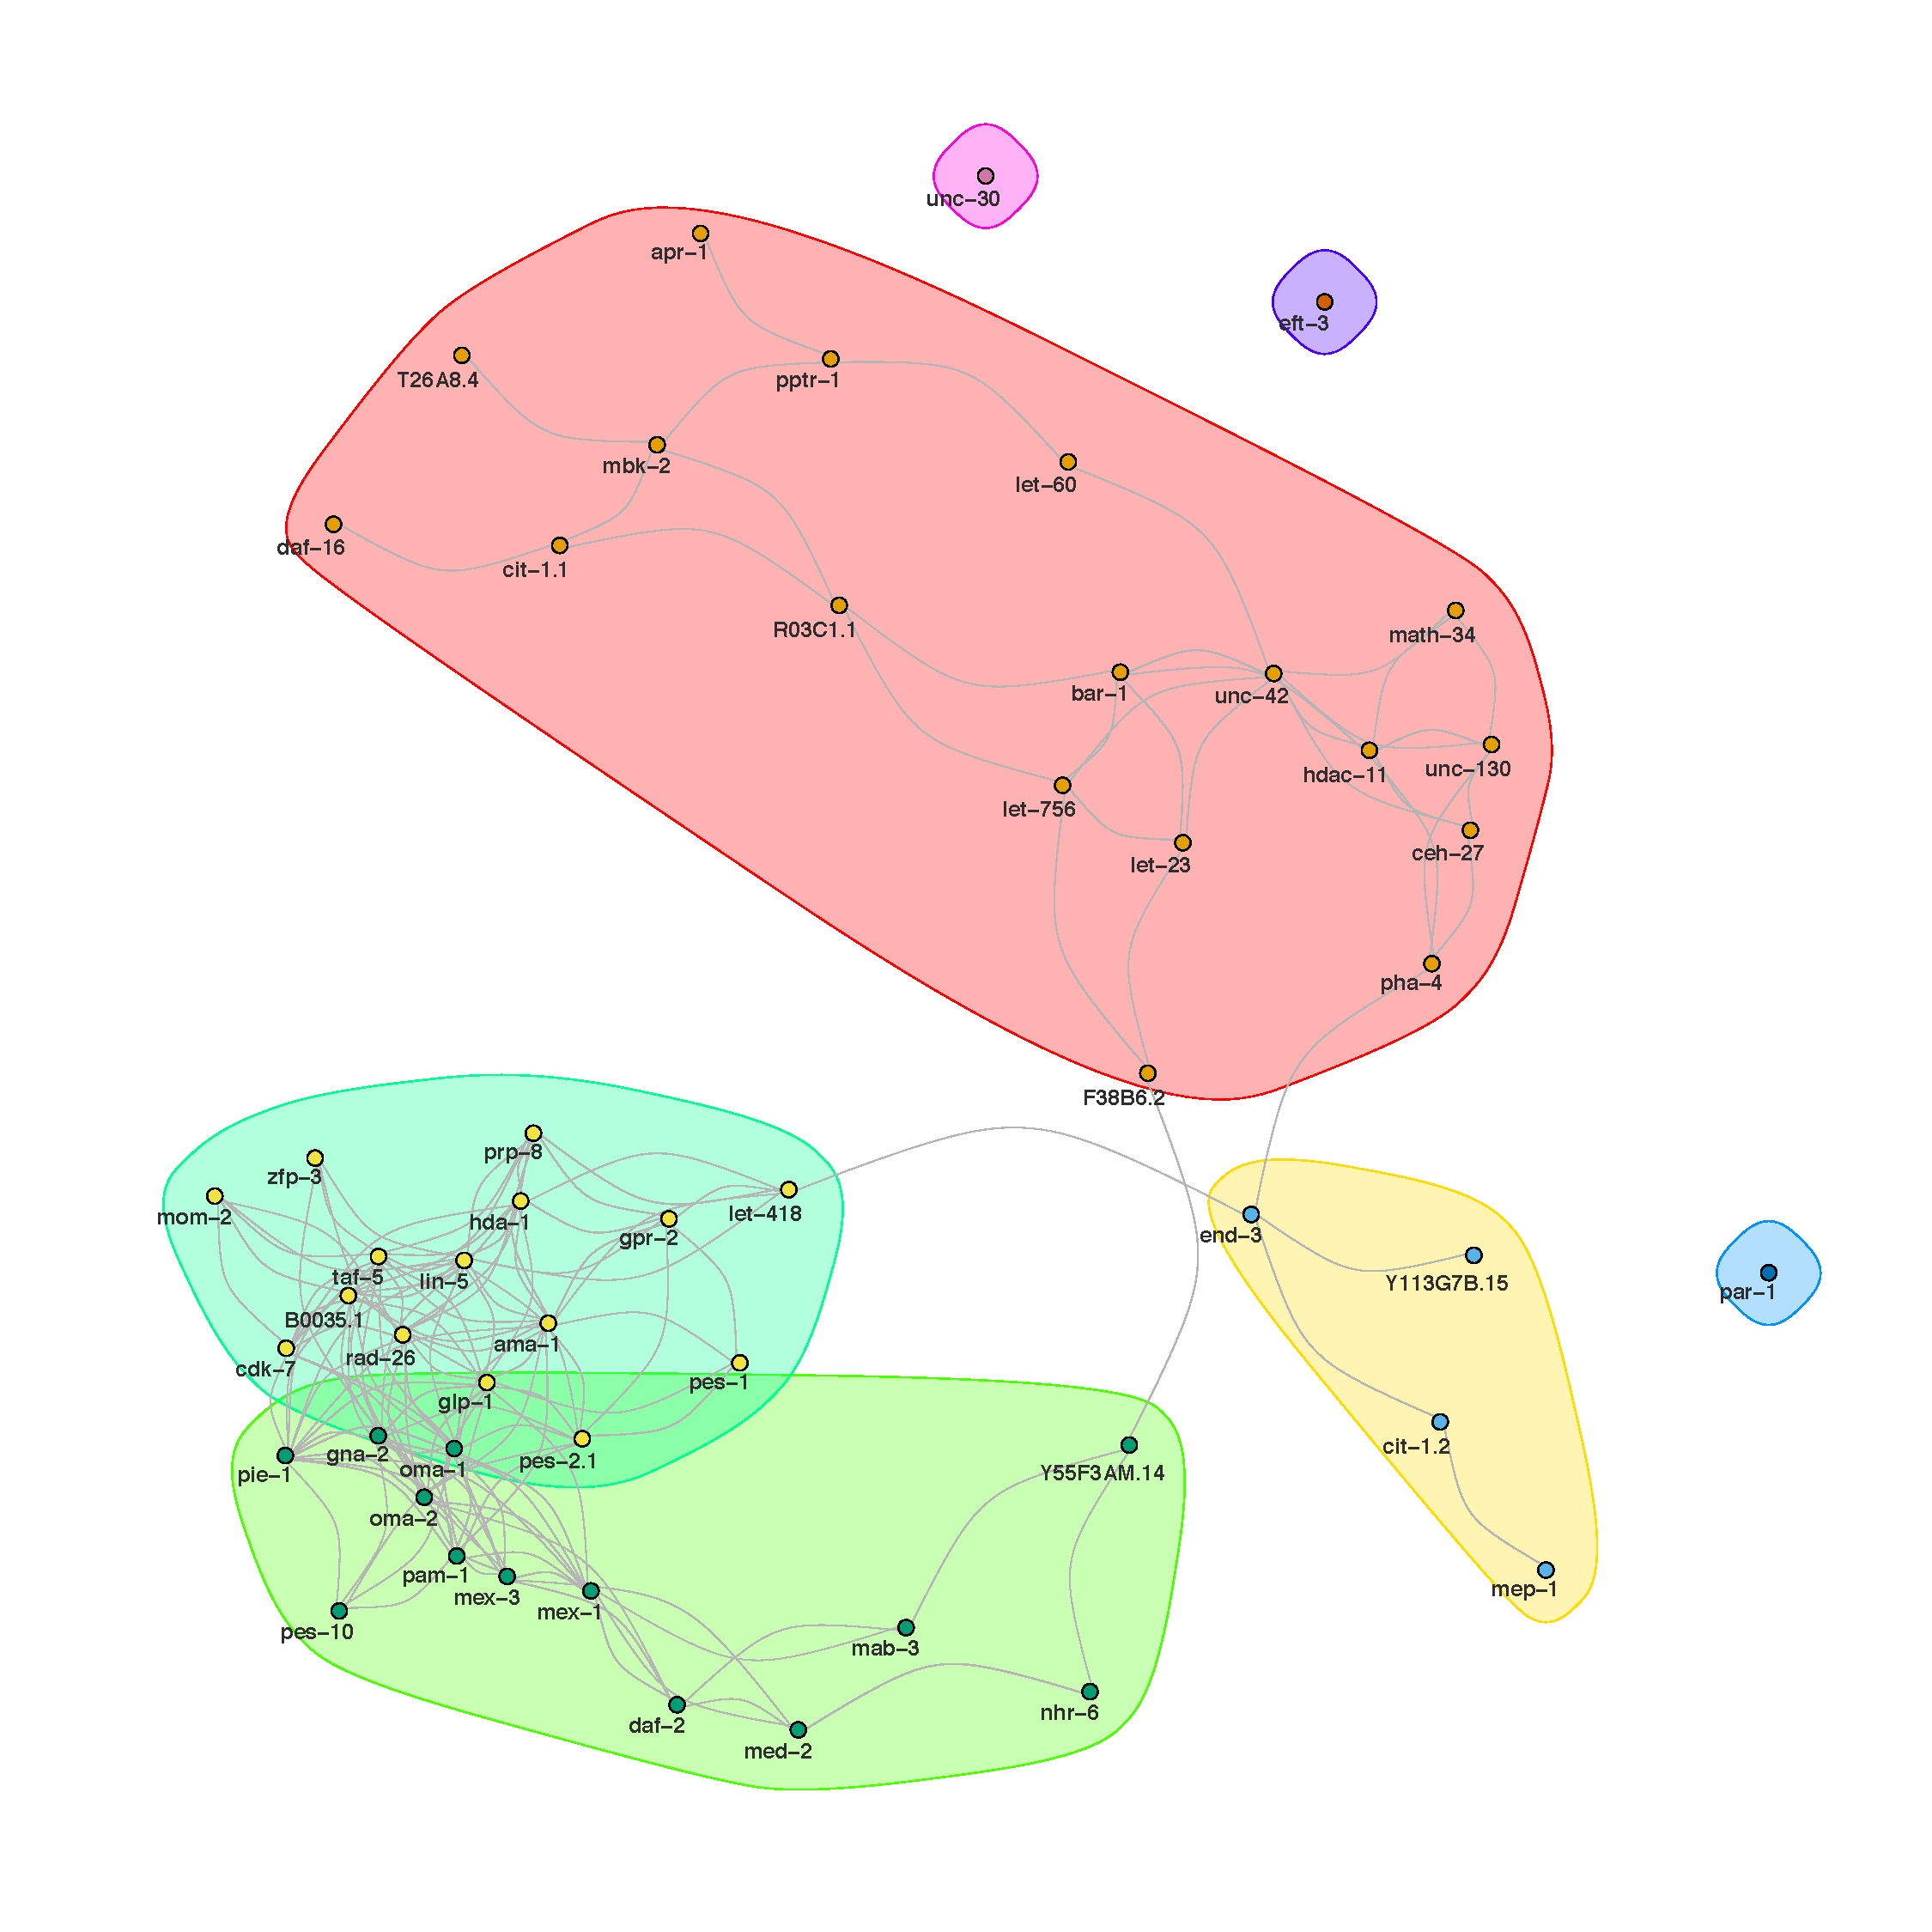
\includegraphics[width=\textwidth]{network_pos.pdf}
  \captionof{figure}{\textbf{Network constructed using only positive correlations between 64 candidate genes.}}
  \label{fig:network_pos}
\end{figure}

\begin{figure}[H]
  \centering
    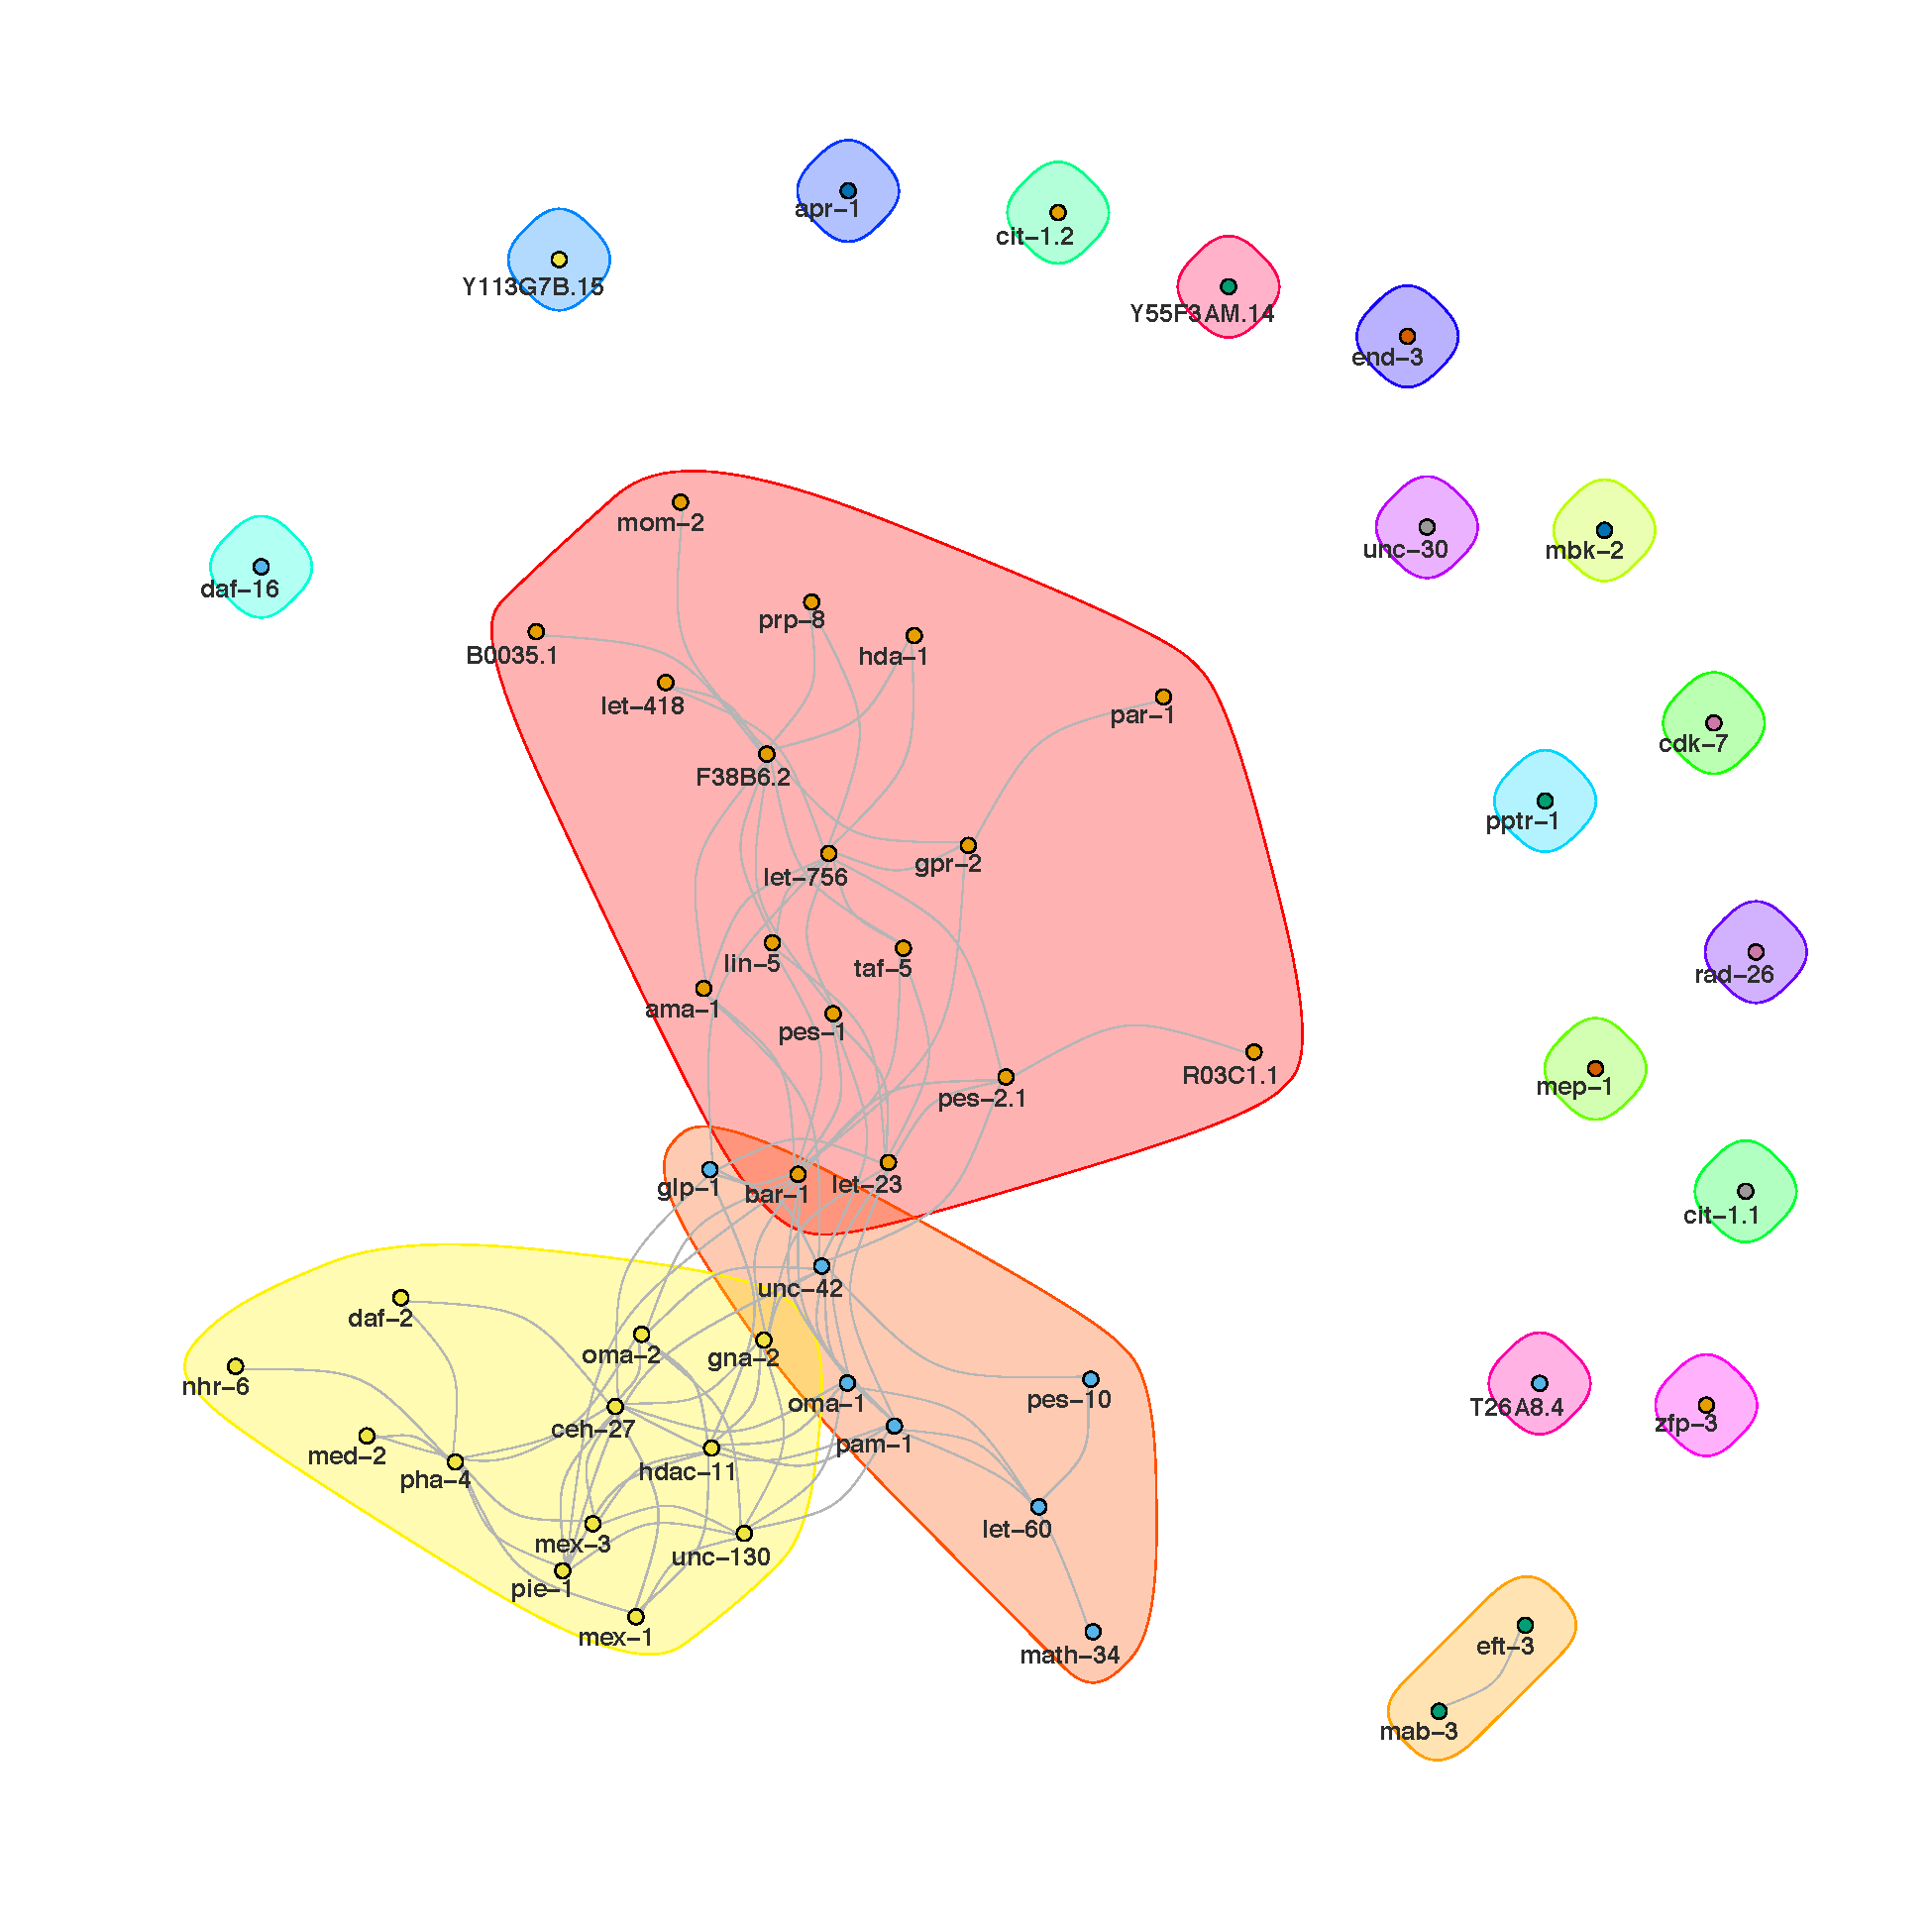
\includegraphics[width=\textwidth]{network_neg.pdf}
  \captionof{figure}{\textbf{Network constructed using only negative correlations between 64 candidate genes.}}
  \label{fig:network_neg}
\end{figure}

\subsection{Genes with expression patterns that correlate strongly with \textit{pie-1}.}

\subsubsection{Postively correlated gene expressions}
In the positive correlations network~(\autoref{fig:network_pos}), 12 genes were found in the community containing \textit{pie-1}. The gene expression data of these genes were used to generate another heatmap using Ward's method (ward.D2)~(\autoref{fig:subposheatmap}). 

\begin{figure}[H]
  \centering
    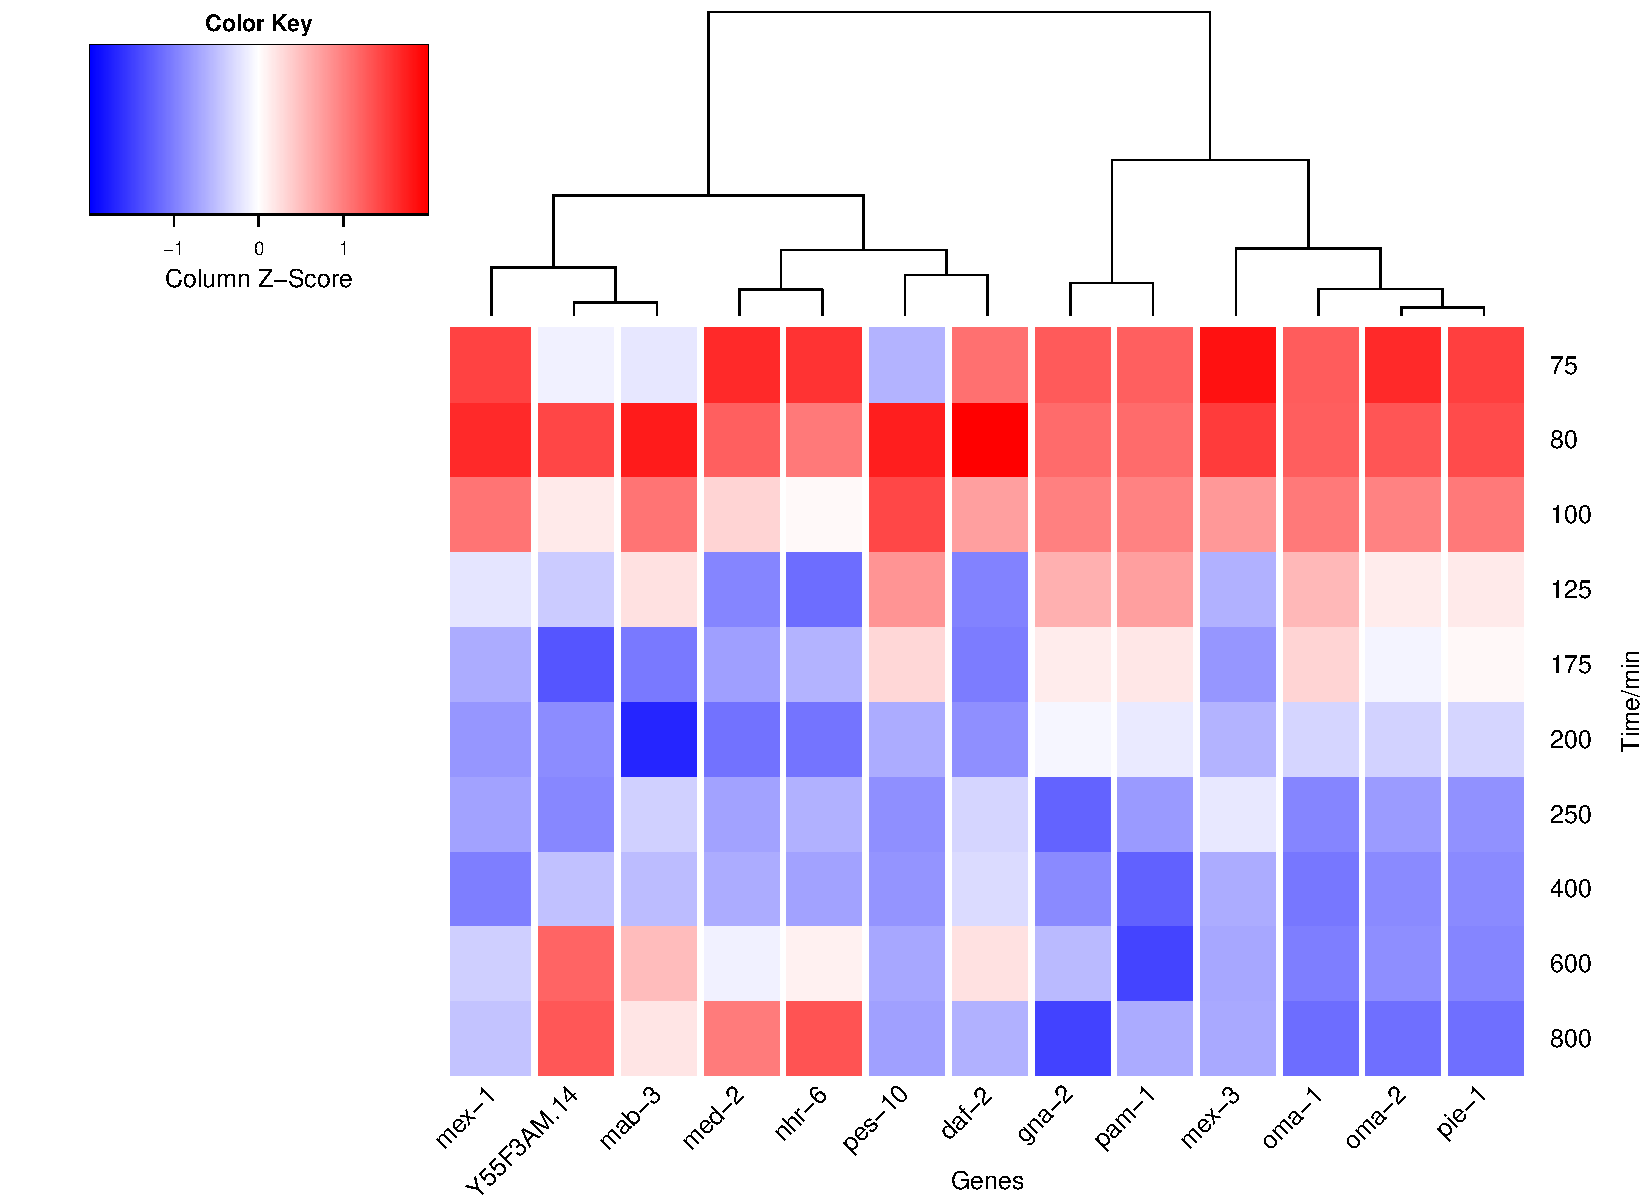
\includegraphics[width=\textwidth]{subposheatmap.pdf}
  \captionof{figure}{\textbf{Heatmap of gene expressions that correlate positively with \textit{pie-1}.}}
  \label{fig:subposheatmap}
\end{figure}

\textit{oma-1, oma-2} and \textit{mex-3} were subsequently selected for further analysis.

\begin{figure}[H]
  \centering
    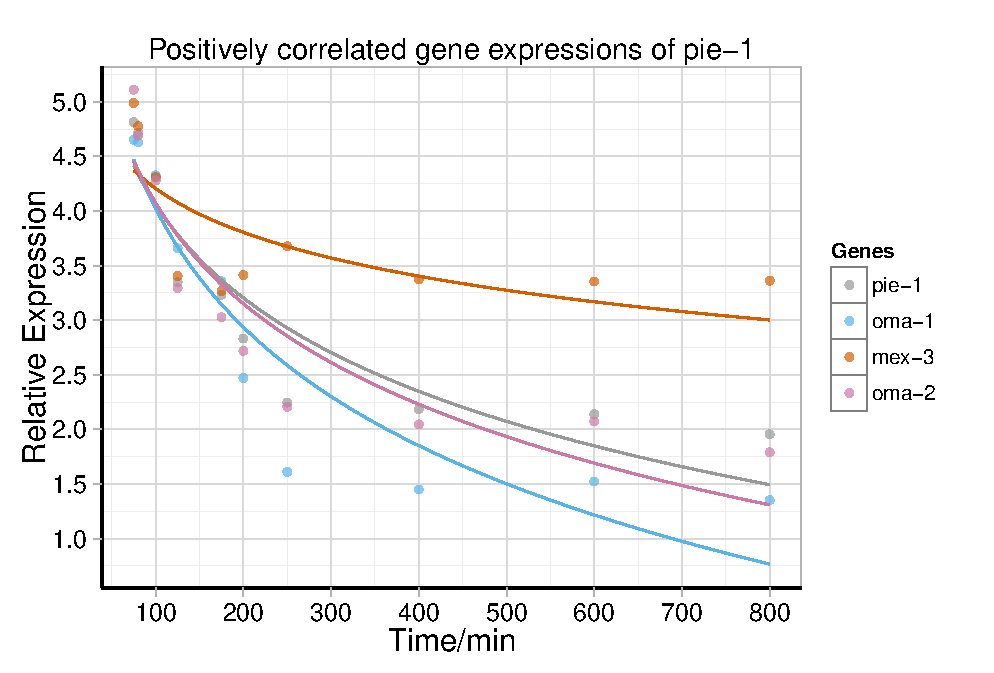
\includegraphics[width=0.7\textwidth]{subposplot.pdf}
  \captionof{figure}{\textbf{Positively correlated gene expressions of \textit{pie-1}.} \footnotesize Time on the x-axis indicates the amount of time since the 4-cell stage. Fitted lines were drawn using an exponential decay model.}
  \label{fig:subposplot}
\end{figure}

All four genes decreases as embryos proceed with their development~(\autoref{fig:subposplot}).  \textit{oma-1, oma-2} and \textit{mex-3} expression data were best fitted with an exponential decay model (oma-1: adj.~r$^2$~=~0.87, intercept~=~11.23$\pm$1.08, slope~=~-1.57$\pm$0.20, both~p$<$0.0001, res. df = 8)(oma-2: adj.~r$^2$~=~0.83, intercept~=~10.19$\pm$1.10 , slope~=~-1.33$\pm$0.20, both~p$<$0.001, res. df = 8)(mex-3: adj.~r$^2$~=~0.49, intercept~=~6.87$\pm$1.00 , slope~=~-0.58$\pm$0.19, both~p$<$0.05, res. df = 8).


\subsubsection{Negatively correlated gene expressions}
In the negative correlations network~(\autoref{fig:network_neg}), 11 genes were found in the community containing \textit{pie-1}. Their relative expression patterns were used to generate another heatmap using Ward's method (ward.D2)~(\autoref{fig:subnegheatmap}).
\smallskip
\begin{figure}[H]
  \centering
    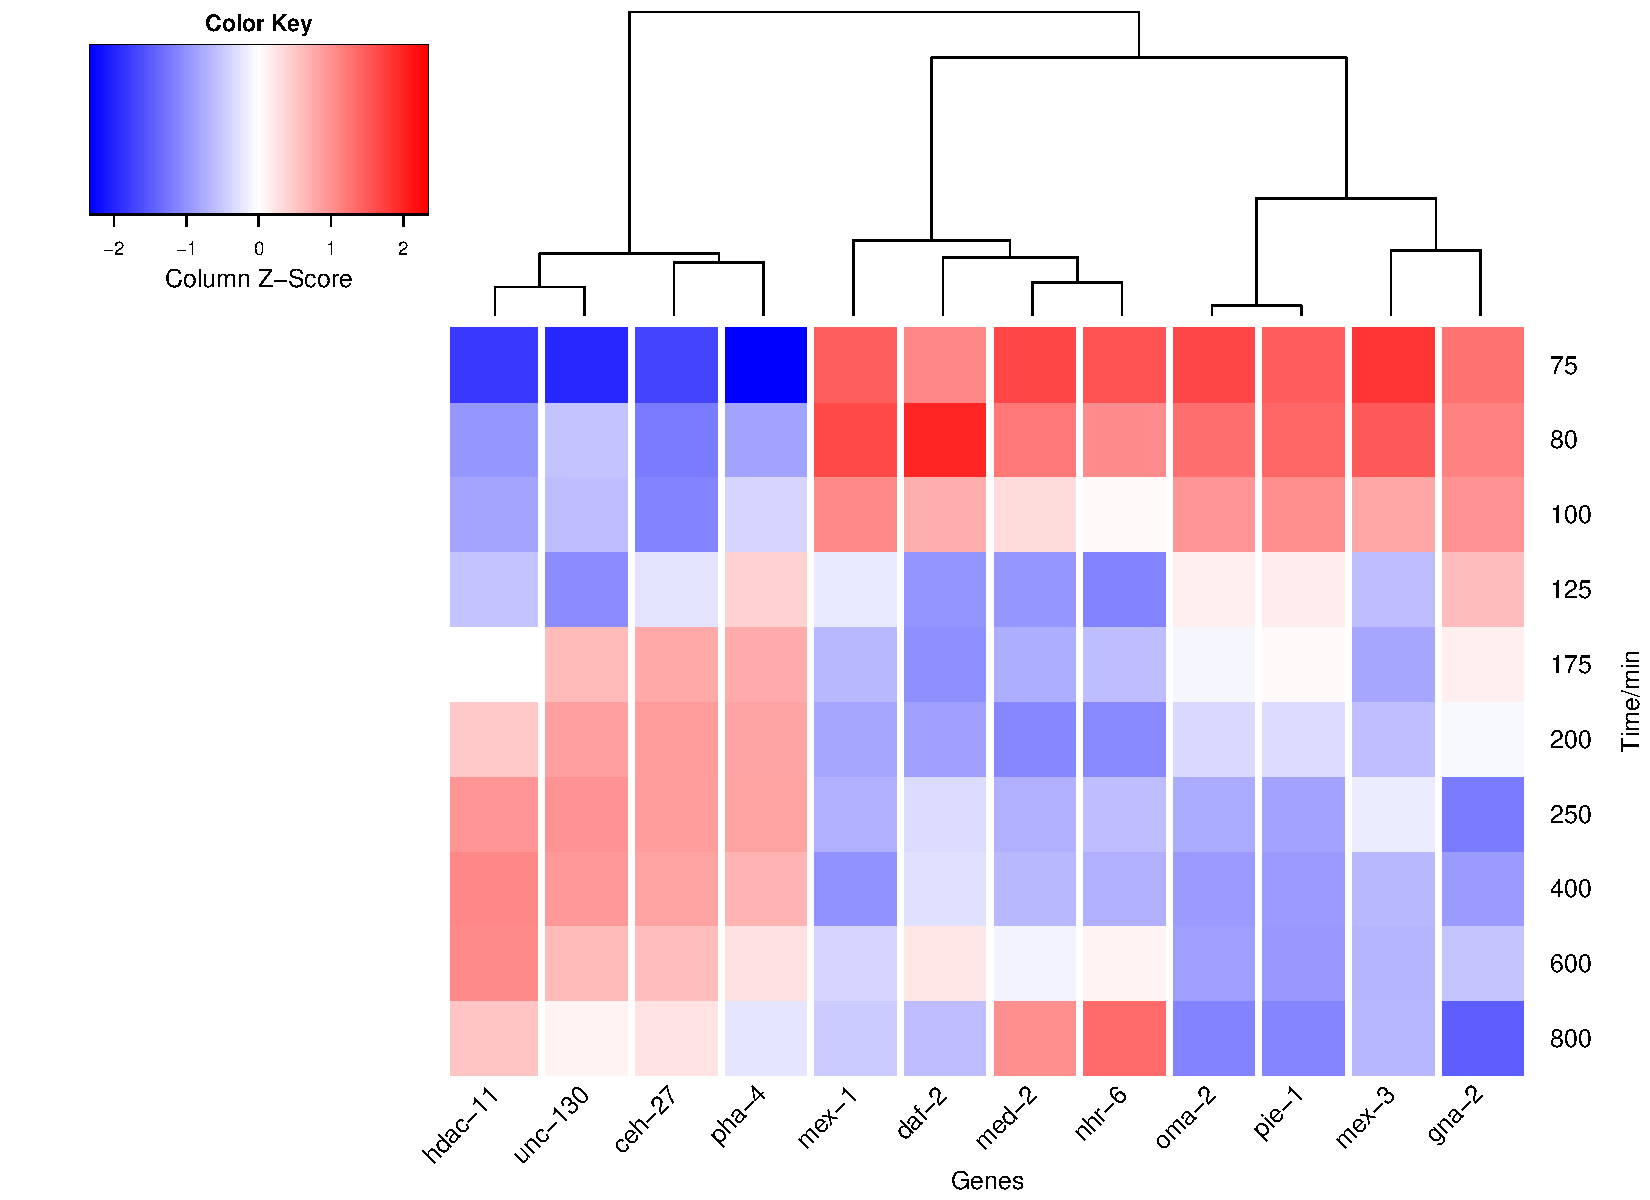
\includegraphics[width=\textwidth]{subnegheatmap.pdf}
  \captionof{figure}{\textbf{Heatmap of gene expressions that correlate negatively with \textit{pie-1}.}}
  \label{fig:subnegheatmap}
\end{figure}

\textit{hdac-11, unc-130, ceh-27} and \textit{pha-4} have gene expression patterns that are the inverse of that of \textit{pie-1} and are possible candidates of inhibition by PIE-1. Thus, these four genes were subsequently used for further analysis.

\begin{figure}[H]
  \centering
    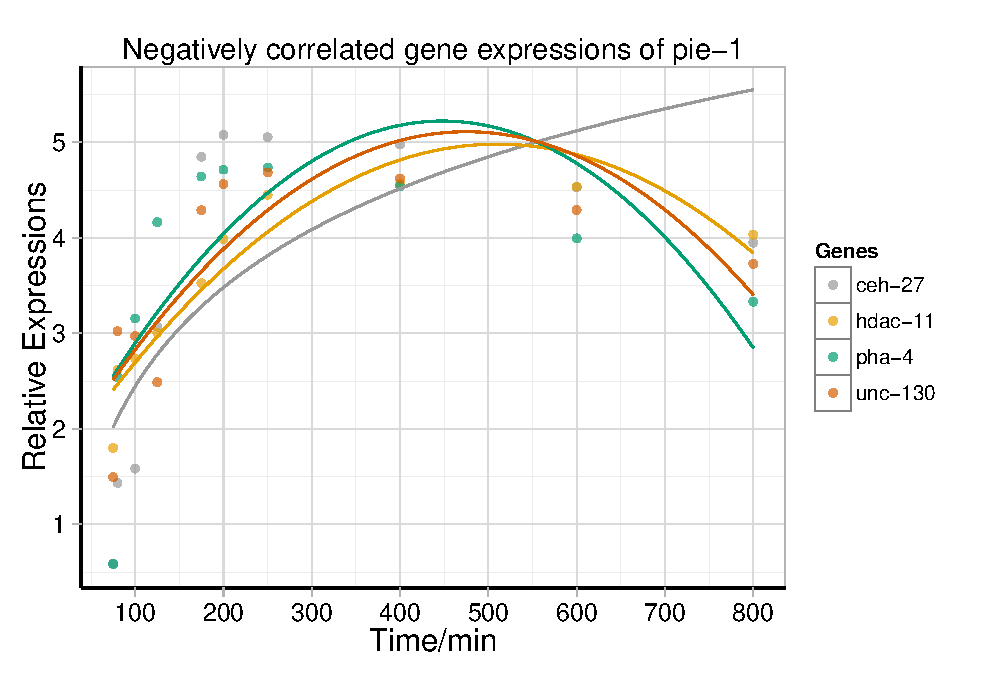
\includegraphics[width=0.8\textwidth]{subnegplot.pdf}
  \captionof{figure}{\textbf{Negatively correlated gene expressions of \textit{pie-1}.} \footnotesize Time on the x-axis indicates the amount of time since the 4-cell stage.}
  \label{fig:subnegplot}
\end{figure}

All four genes have low expression levels at the 4-cell stage and have rapidly increasing expression which peaks at around 200 mins after the 4-cell stage, before expression levels start to fall. \textit{ceh-27} expression levels were best modelled by an exponential decay curve while the expression data of the three other genes were best modelled by a quadratic function. Nonetheless, these models do not represent the data very well, as indicated by low adjusted R values and high p-values~(\autoref{fig:subnegplot}).

\section{Discussion}

\subsection{Postively correlated genes}

\subsubsection{OMA-1 and OMA-2 indirectly activate PIE-1}
Both \textit{oma-1} and \textit{oma-2} (oocyte maturation defective) encode CCCH-type zinc finger proteins and have redundant functions in oocyte maturation in \textit{C. elegans}~\citep{Detwiler2001}. OMA proteins repress transcription globally in the zygote and early germline blastomere by binding to TAF-4, an essential protein in the RNA  polymerase II pre-initiation complex~\citep{Guven-Ozkan2008}.
\\
\\
Another protein, ZIF-1, is a subunit of a E3 ligase that binds to PIE-1 and targets it for degradation. OMA represses translation of \textit{zif-1} by binding to the 5'untranslated region (UTR) of the \textit{zif-1} mRNA, hence preventing the degradation of PIE-1. This indirectly allows transcriptional repression in later germline blastomeres by high levels of PIE-1~\citep{Guven-Ozkan2010}. 
\\
\\
Furthermore, both OMA and PIE-1 are translated from germline-specific maternal RNAs and are associated with P granules, which are granules specific to germ cells~\citep{Shimada2006}. As the ratio of germline cells to somatic cells exponentially decrease as the embryos develop, this may explain the exponential decay in gene expressions. Moreover, \textit{oma-1, oma-2} and \textit{pie-3} have similar gradient values and this could be a result of these genes being regulated together as they have such similar functions~(\autoref{fig:subposplot}).

\subsubsection{\textit{mex-3}}
\textit{mex-3} (muscle excess) encodes another maternally produced CCCH-type zinc finger protein. \textit{mex-3} mutants give birth to embryos with excess muscle and hypodermal cells, resulting in a lethal phenotype~\citep{Pagano2009}. Its protein, MEX-3,  acts as a translational repressor by binding to MEX-3 recognition elements (MREs) found in the 3'UTR of several transcripts such as \textit{pal-1}, hence maintaining the pluripotency of germline cells, where it accumulates~\citep{Pagano2009}. However, it remains unknown if \textit{pie-1} mRNA contains any MREs.
\\
\\
Similar to OMA, MEX-3 is a RNA-binding protein that is associated with P granules and act as a repressor of ZIF-1~\citep{Draper1996, Oldenbroek2012}, which may explain its similar trend of expression with that of \textit{oma-1, oma-2} and \textit{pie-1}~(\autoref{fig:subposplot}). 

\subsection{Negatively correlated genes}
HDAC-11, UNC-130, CEH-27 and PHA-4 were found to interact with PIE-1 in a recent study using enhanced yeast one-hybrid and two-hybrid assays~\citep{Reece-Hoyes2013}. Moreover, community detection algorithm in the network with negative correlations placed the four genes that encode these proteins in the same community as PIE-1, further supporting the hypothesis that PIE-1 inhibits these proteins or genes. Nonetheless, there has been no further papers that have looked into the interaction between these four proteins and PIE-1.

\subsubsection{\textit{hdac-11} may regulate somatic neural differentiation.}
Histone deacetylase-11 (HDAC-11), encoded by \textit{hdac-11}, is an ortholog of the human HDAC11 protein. The human HDAC11 protein is enriched in oligodendrocytes and has been shown to be important in oligodendrocyte development~\citep{Liu2009}. However, there has been no further research conducted regarding the \textit{hdac-11} gene in \textit{C. elegans}. Nonetheless, histone deacetylases play essential roles in suppressing and enhancing transcription across several locations in the genome by the modification of histones~\citep{Gregoretti}. Hence, it is possible that a key germline transcription factor such as PIE-1, may inhibit either directly or indirectly the expression of \textit{hdac-11}, thereby suppressing the expression of somatic neural differentiation genes. 

\subsubsection{\textit{unc-130} is responsible for the formation of olfactory neurons.}
\textit{unc-130} (uncoordinated-130) encodes a evolutionarily conserved Forkhead Box transcripition factor that can activate or repress transcription of other genes. This group of transcription factors play multiple complex roles in metazoan development, hence making it difficult to elucidate their functions. In \textit{C.elegans}, UNC-130 participates in the formation of olfactory neurons as well as in the formation of mesoderm patterning~\citep{Kersey2016, Nash2000, Sarafi-Reinach2000}. Similarly, PIE-1 may suppress theis gene expression to maintain pluripotency of germline cells.

\subsubsection{\textit{pha-4} participates in the organogenesis of the pharynx.}
The \textit{pha-4} gene is expressed during embryonic development, producing a FoxA transcription factor that acts as a organ identity factor. PHA-4 is crucial in the development of the pharynx in \textit{C.elegans}~\citep{Mango1994}. As PIE-1 maintains germline cell fate, it is likely that it participates in the inhibition of \textit{pha-4} inhibition.

\subsubsection{Functions of \textit{ceh-27} remain unclear.}
\textit{ceh-27} is crucial for embryogenesis and seems to be involved in the maintenance of hypodermal integrity. However, the functions of CEH-27 remains unclear as little research regarding the protein itself has been conducted.

\section{Further Research}
Many of the gene products discussed in this report are primarily accumulated in the germline blastomeres. Hence, it would be interesting to compare the transcriptomics of germline blastomeres to that of somatic blastomeres to elucidate other genes that are enriched in germline blastomeres. Such genes may display a highly correlated expression with \textit{pie-1}  and may not have been identified in this practical as expression levels were averaged throughout the embryonic cells. 
\\
\\
Although statistical analysis of gene expressions is able to highlight significant correlations between gene expression patterns, additional supporting data will be needed before these gene interactions can be proven true. Moreover, further cell assays will be required to elucidate the molecular mechanisms behind such gene interactions. 
\\
\\
Lastly, by researching on key embryonic transcription factors such as PIE-1 in \textit{C. elegans}, we can gain a better understanding of the molecular mechanisms behind the maintenance of pluripotency and embryonic development. As there are many conserved pathways between the two species~\citep{Kaletta2006}, using \textit{C. elegans} as a model to understand human embryonic development is hence a useful tool.


\newpage
\bibliography{pie}
\bibliographystyle{cell}

\end{document}


